%%%%%%%%%%%%%%%%%%%%%%%%%%%%%%%%%%%%%%%%%%%%%%%%%%%%%%%%%%%%%%%%%%%%
\documentclass[12pt]{report}
%%%%%%%%%%%%%%%%%%%%%%%%%%%%%%%%%%%%%%%%%%%%%%%%%%%%%%%%%%%%%%%%%%%%
\setlength{\textwidth}{6.25in} % original 6.25
\setlength{\textheight}{650pt}
\renewcommand{\baselinestretch}{1.3}

\oddsidemargin 20pt    %  Left margin on odd-numbered pages.
\evensidemargin 20pt   %  Note that \oddsidemargin = \evensidemargin
\topmargin 0pt
%%%%%%%%%%%%%%%%%%%%2%%%%%%%%%%%%%%%%%%%%%%%%%%%%%%%%%%%%%%%%%%%%%%%%
\usepackage {graphics}
\usepackage {epsfig}
\usepackage {graphicx}
\usepackage{fancyhdr}
%\usepackage{fixltx2e}
\usepackage[usenames,dvipsnames]{color}
%%%%%%%%%%%%%%%%%%%%%%%%%%%%%%%%%%%%%%%%%%%%%%%%%%%%%%%%%%%%%%%%%%%%
%\pagestyle{empty}
\begin{document}

\pagenumbering{gobble}
\pagestyle{fancyplain}
\fancyhf{}
\rhead{\fancyplain{}{\thepage}}

\thispagestyle{empty}
\textbf{\hspace{55mm} \large Assignment 1}\\
\begin{enumerate}
\textbf{\hspace{35mm}  Knowledge canvas and IDEA Matrix }\\

\hspace*{0.325 in} Knowledge canvas is one that depicts the knowledge forces and knowledge flow across organization and extended organizations. It captures the current knowledge state and knowledge forces in the environment. It tries to build bigger and broader knowledge scenario for user and system environment. \\
\hspace*{0.3 in}Principle component for knowledge canvas for hand gesture recognition system are:\\
1.	Knowledge force for cost saving\\
2.	Knowledge about precision\\
3.	Knowledge about nearby interaction\\
4.	External knowledge forces\\
5.	Location based event awareness\\
\begin{figure}[h]
\centering
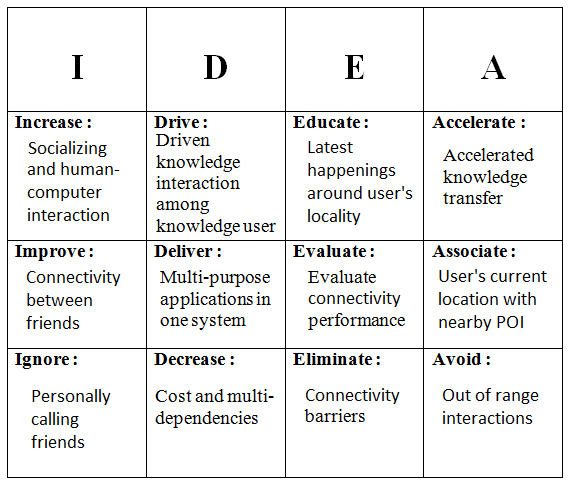
\includegraphics[scale=0.7]{idea.png}
\caption{IDEA Matrix Framework}
\end{figure}
\end{enumerate}
\item\textbf{Software and Hardware Specification:}
\begin{enumerate}
\item \textbf{Hardware Specification:}
\begin{enumerate}
\item Android Smartphone
\item Memory of 1 GB RAM (or more) in android phone
\end{enumerate}
\item \textbf{Software Interface:}
\begin{enumerate}
\item Front end : Android
\item Back end : Parse Cloud
\item Android studio
\item Android sdk tools
\item Java SE JDK 1.7
\end{enumerate}
\item\textbf{Technologies Used:}\\
\begin{enumerate}
\item\textbf{Android}\\
   Android is an operating system for mobile devices. It is mostly used for cell phones, like Google's own Galaxy Nexus, as well as by other phone manufacturers like HTC and Samsung. It has also been used for tablets such as the Motorola Xoom and Amazon Kindle Fire. Android's kernel is based on Linux. Programs for Android, also called "apps", come from the Google Play store. The android programs have an extention of .apk. Android programs are built in C, C++, or Java programming languages but the UI is always made using Java. There are over 900,000 apps available for Android. Each version of Android has both a number and a name based on a dessert. The version numbers and names are:
   \begin{enumerate}
      
    \item Beta versions: Astro and Bender
    \item 1.5: Cupcake
    \item 1.6: Donut
    \item 2.0 and 2.1: Eclair
    \item 2.2: Froyo (FROzen YOgurt)
    \item 2.3: Gingerbread
    \item 3.x: Honeycomb (a tablet-only version)
    \item 4.0: Ice Cream Sandwich
    \item 4.1, 4.2 and 4.3: Jelly Bean
    \item 4.4: KitKat
    \item 5.0: Lollipop
    \item 6.0: Marshmallow
    
    \end{enumerate}
\textbf{Features in the Android operating system :} \\
1. Messaging\\
2.Web browser\\
3. Voice-based features\\
4. Multitasking\\
5. Connectivity\\
6. Media support\\
7. Location based service
\item\textbf{Parse Cloud}\\
   Mobile Backend as a Service(MBaaS), also known as ``backend as a service" (BaaS), is a model for providing web and mobile app developers with a way to link their applications to backend cloud storage. The Parse Android SDK allows you to store data, manage users, send push notifications, track analytics, and more in just a few lines of code. Keep your users engaged and coming back for more with Parse Push. Create highly effective push campaigns with just a few clicks and measure their success with Parse Analytics. With a single line of code, track any data point in your app using Parse Analytics. View app usage, push campaigns, and custom analytics in the user-friendly Parse dashboard. Overlay graphs, filter by date, and more to gain insight into the effectiveness of your app.
   
\item\textbf{Location based service}\\
	A location-based service (LBS) is a software application for a IP-capable mobile device that requires knowledge about where the mobile device is located. Location-based services can be query-based and provide the end user with useful information such as "Where is the nearest ATM?" or they can be push-based and deliver coupons or other marketing information to customers who are in a specific geographical area.\\
\end{enumerate}
\end{enumerate}
\end{enumerate}
\pagebreak
\textbf{\hspace{55mm} \large Assignment 2}\\
\\
\begin{flushleft}
\textbf{\ Project problem statement}\\
\end{flushleft}
\\
\begin{enumerate}
\item\textbf{Feasibility assessment using NP-Hard, NP-Complete or satisfiability issues using modern algebra}\\
\\
\textbf{Problem Definition}\\
\hspace*{0.3in} Recommending friends instantly based on current location of users in the real world has become increasingly popular in Location-based mobile social network (LMSN). However, the existing friend recommendation methods based on topological structures of a social network or non-topological information such as similar user profiles cannot well address the instant making friends in the real world.\\
\\

\begin{enumerate}
\item\textbf{Problem :} Calculate distance between any two friends.\\
\item\textbf{Input : } Latitude and Longitude of the all friends in favourites list.
\item\textbf{Output : } Distance is calculated between user and all friends, then if the distance is less than range provided by user then it shows nearest friends on map. 
\end{enumerate}
  
So that problem definition is \textbf{NP-Complete}.\\
\\
\item\textbf{Mathematical model}\\
S is a system for implementing a location based android application.

S = {s, e, x, y, DD, NDD, success, failure, CPU core count} 

s = Start state

e = End state

x = input : Current location

y = output : List of nearby friends

DD = Deterministic Data : Current location.

NDD = Non-Deterministic Data : User interest based suggestions, range, nearby friends.

Success case : List of all nearby friends within the range.

Failure case : GPS is disabled

CPU core count = No. of cores required to execute the application : 1
\\
\hspace*{0.5in}A representation in mathematical terms of the behaviour of real devices and objects. A mathematical model is a description of a system using mathematical concepts and language. The process of developing a mathematical model is termed mathematical modelling. Method of simulating real life situations with mathematical equations to forecast their future behaviour. Mathematical modelling uses tools such as decision theory, queuing theory, and linear programming, and requires large amounts of number crunching.
\\
\item\textbf{Need Of Mathematical Model}\\
\hspace*{0.5in} Since the modelling of devices and phenomena is essential to both engineering and science, engineers and scientists have very practical reasons for doing mathematical modelling. In addition, engineers, scientists, and mathematicians want to experience the sheer joy of formulating and solving mathematical problems.\\
\begin{enumerate}
\item Enables a thorough understanding of the system modelled.}
\item Prepares the way for better design or control of the system.}
\item Allows the efficient use of modern computing capabilities.}
\end{enumerate}
\\
\item\textbf{Objective}\\
\begin{enumerate}
\item Locate your friends on Map
\item Chat with friends
\item Create events and suggest users on the basis of their interest
\item Locate interested members for an event on map to properly schedule event
\end{enumerate}

\item\textbf{Outcomes}
\\
\textbf{Success:}
Locate the near-by users within a given range.
\\
\textbf{Failure:}
GPS is not enabled, so unable to locate users current location.
\\
\end{enumerate}
\\
\\
\pagebreak
\textbf{\hspace{55mm} \large Assignment 3}\\
\\
\begin{flushleft}
\textbf{\ Distributed/parallel/concurrent processing}\\
\end{flushleft}
\begin{enumerate}
\item\textbf{Domian Information :}
\begin{enumerate}
\item\textbf{Location Based Service (LBS):}
\hspace*{0.5}Location-based services (LBS) are a general class of computer program-level services that use location data to control features. As such LBS is an information service and has a number of uses in social networking today as an entertainment service, which is accessible with mobile devices through the mobile network and which uses information on the geographical position of the mobile device. \\
\hspace*{0.5in}A location-based service (LBS) is a software application for a IP-capable mobile device that requires knowledge about where the mobile device is located. Location-based services can be query-based and provide the end user with useful information such as "Where is the nearest ATM?" or they can be push-based and deliver coupons or other marketing information to customers who are in a specific geographical area. An LBS requires five basic components: the service provider's software application, a mobile network to transmit data and requests for service, a content provider to supply the end user with geo-specific information, a positioning component (see GPS) and the end user's mobile device. By law, location-based services must be permission-based. That means that the end user must opt-in to the service in order to use it. In most cases, this means installing the LBS application and accepting a request to allow the service to know the device's location.\\
\hspace*{0.5in}Although location-based services have been around since 2000, they have mostly been used in commerce with a subscription-based business model. The release of Apple's 3G iPhone and Google's LBS-enabled Android operating system, however, has allowed developers to introduce millions of consumers to LBS. According to the 2008 fourth-quarter report from Nielsen Mobile, a division of The Nielsen Company, location-based services account for 58 percent of the total downloaded application revenue for mobile phones in North America.\\
\end{enumerate}
\\
\item\textbf{Implementation Plan }\\
Phase I\\
\begin{figure}[hbtp]
\centering
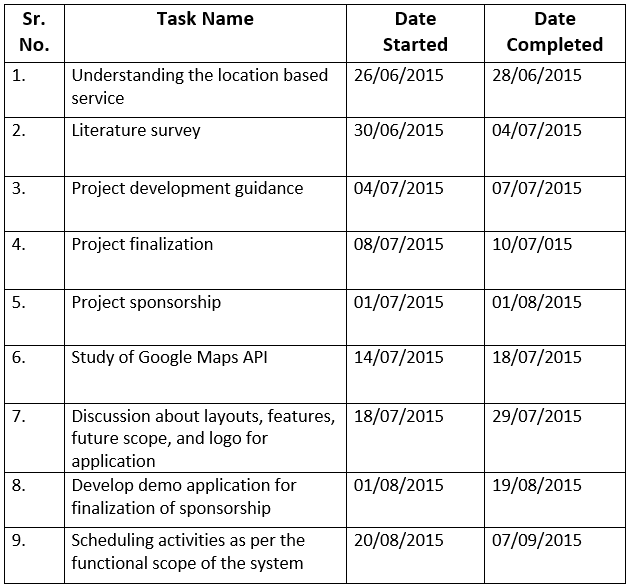
\includegraphics[scale=0.775]{implementationPlan.png}
\caption{System implementation plan phase 1}
\end{figure}\\
\pagebreak
\item\textbf{Team Structure}\\
\begin{figure}[hbtp]
\centering
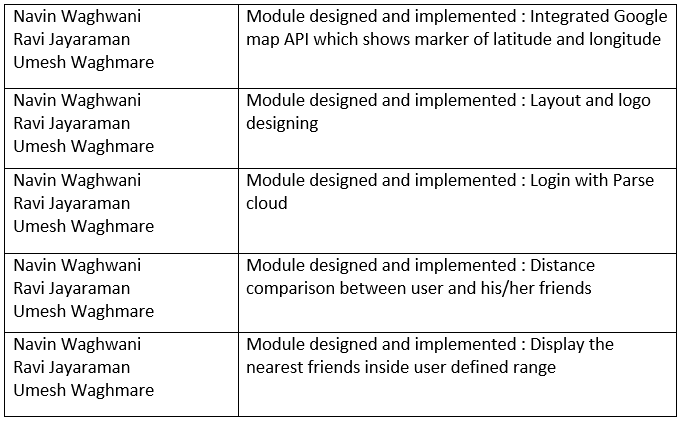
\includegraphics[scale=0.825]{teamStructure.png}
\caption{Team structure}
\end{figure}\\
\\
\\
\pagebreak
\\
\hspace*{2.125 in}\textbf{\large Assignment 4}\\
\begin{flushleft}
\textbf{\ Software modelling methods}\\
\end{flushleft}

\begin{enumerate}
\item DFD
\item To draw functional dependency graphs and relevant, techniques including UML diagrams or other necessities using appropriate tools.
\begin{enumerate}
\item\textbf{Data Flow Diagrams}  \\
\textbf{Level 0 DFD} \\
\hspace*{0.5in}It is common practice to draw the context level DFD first, which shows the interaction between the system and user. On the context diagram the systems interactions with the outside world are modeled purely in terms of data flows across the system boundary. The diagram shows the entire system as a single process. The Level 0 DFD shows how the system is divided into sub-systems (processes), each of which deals with one or more of the data flow to or from an user and data owner, and which together provide all of the functionality of the system as a whole.\\
\hspace*{0.5in} The DFD level 0 shows a simple implementation for the system in which system takes input and pre process the image and simply convert into clear output.\\
\\
\begin{figure*}[h]
\centerline{\psfig{figure=DFD-0.png,width=8.5 cm,height=5.26 cm}}
\label{atcres}
\caption{level 0 DFD}
\end{figure*}
\\
\textbf{Level 1 DFD} \\


\hspace*{0.5in} The Level 1 DFD shows various steps for generating a clear document image from the degraded image.The image is first converted into gray scale.then the image segmentation algorithm is applied and the post processing is done to convert the image into clear document image.\\

\begin{figure*}[h]
\centerline{\psfig{figure=DFD-1.png,width=8.5 cm,height=5.26 cm}}
\label{atcres}
\caption{level 1 DFD}
\end{figure*}
\\

\item Class Diagram\\
\hspace*{0.5in}Class Diagram is a type of static structure diagram that describes the structure of a system by showing the systems classes, their attributes, and the relationships between the classes. Class diagrams are the backbone of almost every object oriented methods, including UML. They describe the static structure of a system. An object Class describes a group of objects with similar properties (attributes), common behaviour (operations),common relationships to the other objects, and common semantics.\\

\\
\begin{figure*}[h]
\centerline{\psfig{figure=Class_diagram.png,width=8.5 cm,height=5.26 cm}}
\label{atcres}
\caption{Class Diagram}
\end{figure*}
\\

\begin{figure*}[h]
\centerline{\psfig{figure=Uml.png,width=9 cm,height=7.2 cm}}
\label{atcres}
\caption{UML Diagram}
\end{figure*}
\\

\begin{figure*}[h]
\centerline{\psfig{figure=Activity.png,width=10 cm,height=10.5 cm}}
\label{atcres}
\caption{Activity Diagram}
\end{figure*}

\end{enumerate}
\end{enumerate}
\\
\\
\vspace*{5in}
\pagebreak
\\
\vspace*{6in}
\\
\hspace*{2.125 in}\textbf{\large Assignment 5}\\
\hspace*{2.125 in}\textbf{\large Assignment 5}\\
\begin{flushleft}
\textbf{\ Testing of project problem statement}\\
\end{flushleft}

\begin{enumerate}
\item Test data (using mathematical models, GUI, Function testing principles, if any) 
\item Selection and appropriate use of testing tools, testing of UML diagram's reliability.
\end{enumerate}
\\
\textbf{Introduction:} Software testing is the process of executing a program or system with the intent of finding errors. Or it involves any activity aimed at evaluating an attribute or capability of the system and determining that it meets its required results. Software is unlike other physical processes where inputs are received and outputs are produced. Where software differs is in that manner in which it fails. Most physical systems fail in a fixed set of ways. By contrast, software can fail in bizarre ways. Detecting all of the different failure modes for software is generally infeasible. Testing is performed for following purposes: 1. To improve quality 2. For verification and validation Basic software testing.\\ 
\\
\textbf{Phases of software development:}\\
 -Analysis\\
 -Design\\
 -Coding\\
 -Testing\\

\begin{enumerate}
\item\textbf{Test Case}
\begin{figure}[h]
\begin{center}
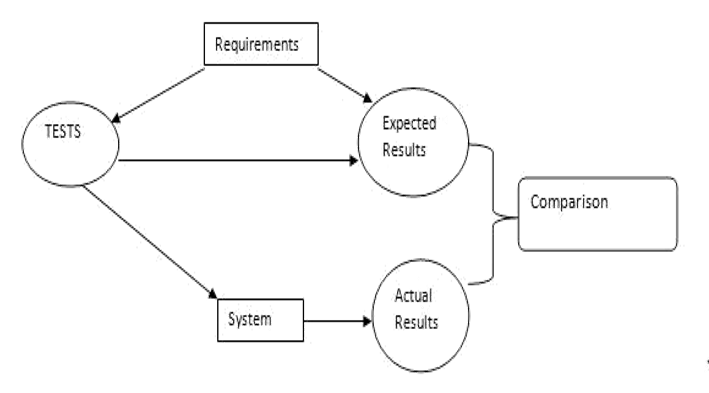
\includegraphics[scale=0.75]{testing.png}
\caption{Framework Of Test Cases}
\end{center}
\end{figure}\\
\begin{enumerate}
\item\textbf{Black Box Testing}
     Black Box Testing is testing without knowledge if internal working of the item being tested. For Example when black box testing is applied to software engineering, the tester would only know the "legal" input and what the excepted output should be, but not how the program actually arrive at those output. It is because of this that black box testing can be considered testing with respect to the specifications, no other knowledge of the program is necessary. For this reason, the tester and the programmer can be independent of the one another, avoiding programmer bias toward his own work. Foe this testing, test group are often used. For glass box testing, the test cases cannot be determined until the code has actually been written. Both of these testing techniques have advantages and disadvantages, but when combine, they help to ensure through testing of the product.\\
Testing methods where user is not required:\\
-Functional: In this type of testing, the software is tested for the functional requirements. The tests are written in outer to check if the application behaves as expected.\\
-Stress: The application is tested against heavy load such as complex numerical values, lager number inputs, large number of queries etc. which check for the stress/load the application can withstand.\\
\item\textbf{White Box Testing}
White box testing strategy deals with the internal logic and structure of the code. White box testing is also called as glass, structure, open box or clean box testing. The tests written based on the white box testing strategy incorporate coverage of the code written. Order to implement white box testing, the tester has to deal with the code and hence is needed knowledge of coding and logic i.e. internal working of the code.\\
Types of testing white/glass box testing strategy:\\
-Unit Testing: The developer carries out unit testing in order to check if the particular module or unit of code is working fine. The unit testing comes at the very basic level as it is carried out as and when the code is developed or a particular functionality is built.\\
-Static and Dynamic Analysis: Static analysis involves going through the code in order to find out any possible defect in the code. Dynamic analysis involves executing the code and analysing the output.\\
-Security Testing: Security Testing is carried out to find out how well the system can protect itself from unauthorized access, hacking cracking, any code damage etc. which deals with the code of application. This type of testing needs sophisticated testing techniques.\\
\\
\item\textbf{Test Plans}\\


\begin{figure*}[h]
\centerline{\psfig{figure=testCases.png,width=14 cm,height=13 cm}}
\label{atcres}
\end{figure*}
\\
\end{enumerate}
\end{enumerate}
\end{document}